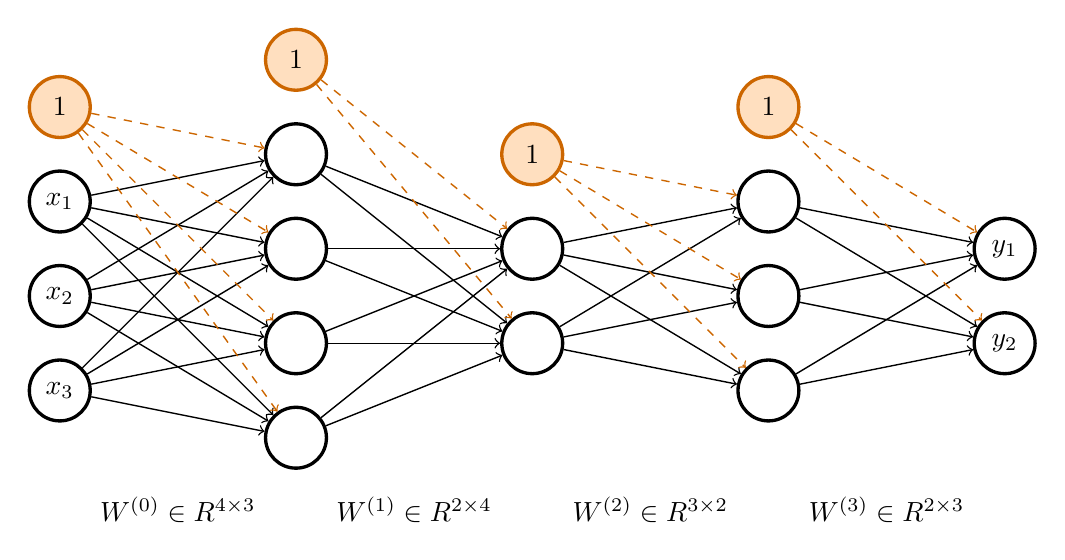
\begin{tikzpicture}[
  neuron/.style={circle, draw, line width=1.2pt, minimum size=22pt, inner sep=0pt},
  input/.style={neuron},
  hidden/.style={neuron},
  output/.style={neuron},
  bias/.style={neuron, draw=orange!80!black, fill=orange!25},
  conn/.style={->, line width=0.5pt},
  bias_conn/.style={->, line width=0.5pt, dashed, orange!80!black}
]

  % Input layer
  \foreach \i/\y in {1/1.2,2/0,3/-1.2} {
    \node[input] (i\i) at (0, \y) {$x_{\i}$};
  }
  \node[bias] (b0) at (0, 2.4) {1};

  % Hidden layer 1
  \foreach \j/\y in {1/1.8,2/0.6,3/-0.6,4/-1.8} {
    \node[hidden] (h1\j) at (3.0, \y) {};
  }
  \node[bias] (b1) at (3.0, 3.0) {1};

  % Hidden layer 2
  \foreach \j/\y in {1/0.6,2/-0.6} {
    \node[hidden] (h2\j) at (6.0, \y) {};
  }
  \node[bias] (b2) at (6.0, 1.8) {1};

  % Hidden layer 3
  \foreach \j/\y in {1/1.2,2/0,3/-1.2} {
    \node[hidden] (h3\j) at (9.0, \y) {};
  }
  \node[bias] (b3) at (9.0, 2.4) {1};

  % Output layer
  \foreach \k/\y in {1/0.6,2/-0.6} {
    \node[output] (o\k) at (12.0, \y) {$y_{\k}$};
  }

  % Connections: Input → Hidden 1
  \foreach \i in {1,...,3} {
    \foreach \j in {1,...,4} {
      \draw[conn] (i\i) -- (h1\j);
    }
  }
  % Add a single weight label, representing the weights matrix
  \node[above] at (1.5, -3) {$W^{(0)} \in \mathbb{R}^{4 \times 3}$};
  
  % Add bias connections
  \foreach \j in {1,...,4} {
    \draw[bias_conn] (b0) -- (h1\j);
  }

  % Connections: Hidden 1 → Hidden 2
  \foreach \i in {1,...,4} {
    \foreach \j in {1,...,2} {
      \draw[conn] (h1\i) -- (h2\j);
    }
  }
  \node[above] at (4.5, -3) {$W^{(1)} \in \mathbb{R}^{2 \times 4}$};
  \foreach \j in {1,...,2} {
    \draw[bias_conn] (b1) -- (h2\j);
  }

  % Connections: Hidden 2 → Hidden 3
  \foreach \i in {1,...,2} {
    \foreach \j in {1,...,3} {
      \draw[conn] (h2\i) -- (h3\j);
    }
  }
  \foreach \j in {1,...,3} {
    \draw[bias_conn] (b2) -- (h3\j);
  }
  \node[above] at (7.5, -3) {$W^{(2)} \in \mathbb{R}^{3 \times 2}$};
  % Connections: Hidden 3 → Output
  \foreach \i in {1,...,3} {
    \foreach \k in {1,2} {
      \draw[conn] (h3\i) -- (o\k);
    }
  }
  \node[above] at (10.5, -3) {$W^{(3)} \in \mathbb{R}^{2 \times 3}$};
  \foreach \k in {1,2} {
    \draw[bias_conn] (b3) -- (o\k);
  }

\end{tikzpicture}
